\documentclass[10pt]{article}
\usepackage{amsmath}
\usepackage{amsfonts}
\usepackage{amssymb}
\usepackage{graphicx}
\usepackage{wrapfig}
\usepackage{commath}

\begin{document}
\section{Introduction} \label{sec:intro}
\par Clamps and "helping hands" are critical tools for skilled, dexterous work. They hold working items like circuit boards steady in a useful position. This seems like an obvious task for a robot - more flexible and user friendly than a purely mechanical solution, but stronger and more tireless than a human assistant. However, the task - holding items to aid dexterous work - has two components which often contradict one another: the grasp needs to hold the object rigidly, but also compliant when necessary. At the same time, it is constrained to avoid certain areas that may be delicate, or in the way of the human. The "Jarvis" project is an attempt to address the problem of providing workplace mechanical assistance in a distributed way - each subproblem is handled by a separate module. 

\par This paper focuses on the Jarvis' perception module, which has two major goals:
\begin{itemize}
\item Identify the human to prevent painful collisions.
\item Identify candidate grasp points on the target.
\end{itemize}

The perception module sends this information to other modules - path planning, human intent, and feasibility. 

\section{Prior Work} \label{sec:prior}

\par Many studies have investigated the problems of robotic grasp selection and human hand-offs. A recent review paper by Bohg et. al.\cite{Bohg2013} gives an overview of state-of-the art grasping approaches and breaks them down into three major categories: grasping known objects, familiar objects, or unknown objects. Grasping completely unknown objects requires 3D reconstruction of an object, tactile feedback,\cite{Hsiao2010} or machine learning on observed features.\cite{Lenz2013}\cite{Saxena}  Our approach lies at the intersection of familiar and unknown grasping.

\par Human interactions and handoffs are often separated from grasp selection. Adding a human to the mix means that the object is no longer sitting still on a flat surface, so detection is harder. Arms and hands constrain the possible grasp points. Micelli et. al. used bounding boxes and partitions based on the human position to move the gripper near the target, but did not select grasp points.\cite{Micelli2011} Many algorithms exist to produce to detect humans and 

\par The plethora of approaches to handoffs and grasping stems from their constraints, with each approach making slightly different assumptions about sensors, known information, and the situation. 

\section{Collision Avoidance} \label{sec:avoidance}
\par The main challenge that the collision avoidance algorithm has to overcome is turning the sensor data into an obstacle that will prevent the path planner from running into the human, while at the same time allowing access to the target item. This rules out pure bounding-box based methods, which are almost always too conservative and would prevent access to the target. Instead, we generate an "arm volume" based on skeleton tracking data. 

\par The collision avoidance algorithm uses the elbow and hand points from the OpenNI skeleton tracking data to generate a vector that points from the elbow to the hand ($\textbf{v}_{eh}$). It then generates a cylinder about this vector to conservatively approximate the volume of the forearm to avoid. This method doesn't specify the entire hand as an obstacle to avoid over-constraining the planner. 

\begin{wrapfigure}{r}{0.5\textwidth}
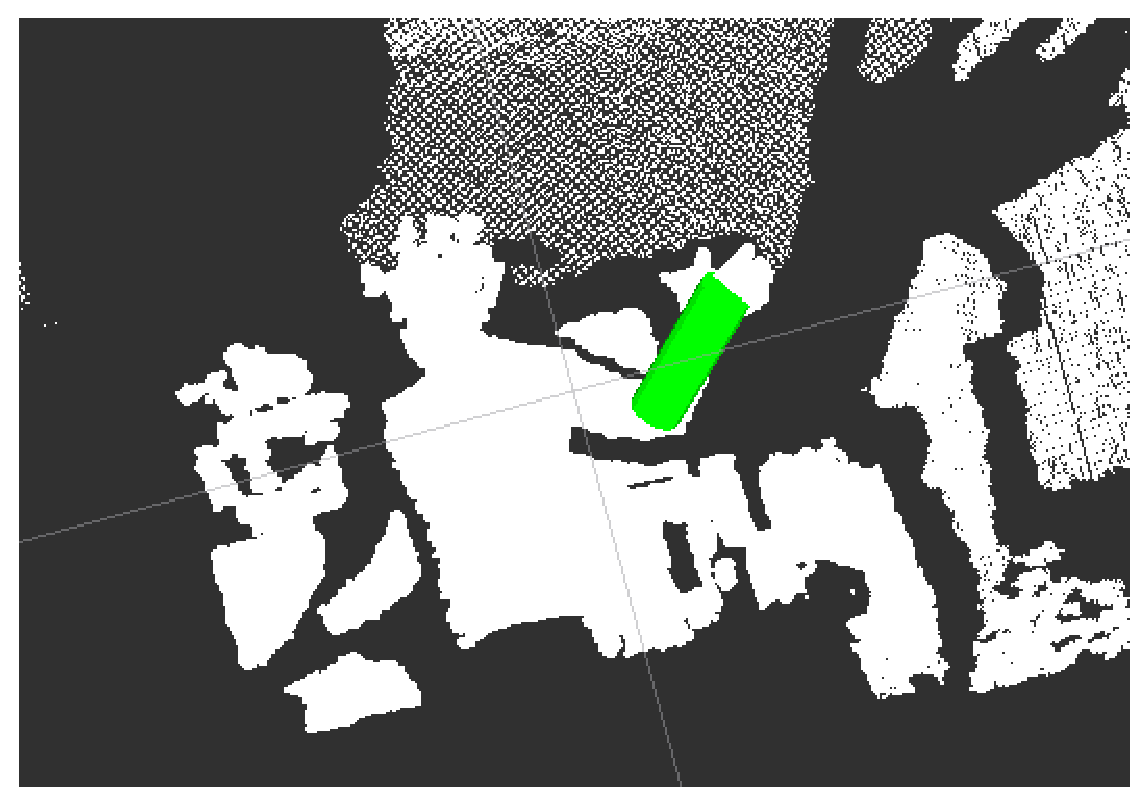
\includegraphics[width=0.48\textwidth]{figures/cropped_arm.eps}  
\caption{Jarvis should avoid the forearm avoidance region shown in green.}
\label{fig:forearm}
\end{wrapfigure}    

\section{Grasp Selection} \label{sec:graspid}
Jarvis uses a three step process to identify the target object and generate possible grasps:
\begin{enumerate}
\item Use the location of the hand and elbow to find a region of interest.
\item Perform a heuristic-based segmentation to generate a point cloud for the target object.
\item Select a grasp based on the target's orientation with respect to the human and its surface normals.
\end{enumerate}
\subsection{Area of Interest Detection} \label{sec:aoi}
The first challenge in selecting a target without a prior model is even knowing where to look - large search spaces increase the probability of misidentifying a heuristically-modeled target. Jarvis takes advantage of the human interaction by assuming the target will be near the human's hand. The area of interest (AoI) is a 0.2 m cube that centers on a target point extended from the hand along the elbow-hand line.  
\par Jarvis respects basic human cuing by checking whether the target is being held towards the robot or not - a common human indication of ``grab this" vs. ``mine!" Jarvis checks whether the elbow or hand is closer to the robot, and only proceeds in the latter case. 

 \begin{wrapfigure}{r}{0.5\textwidth}
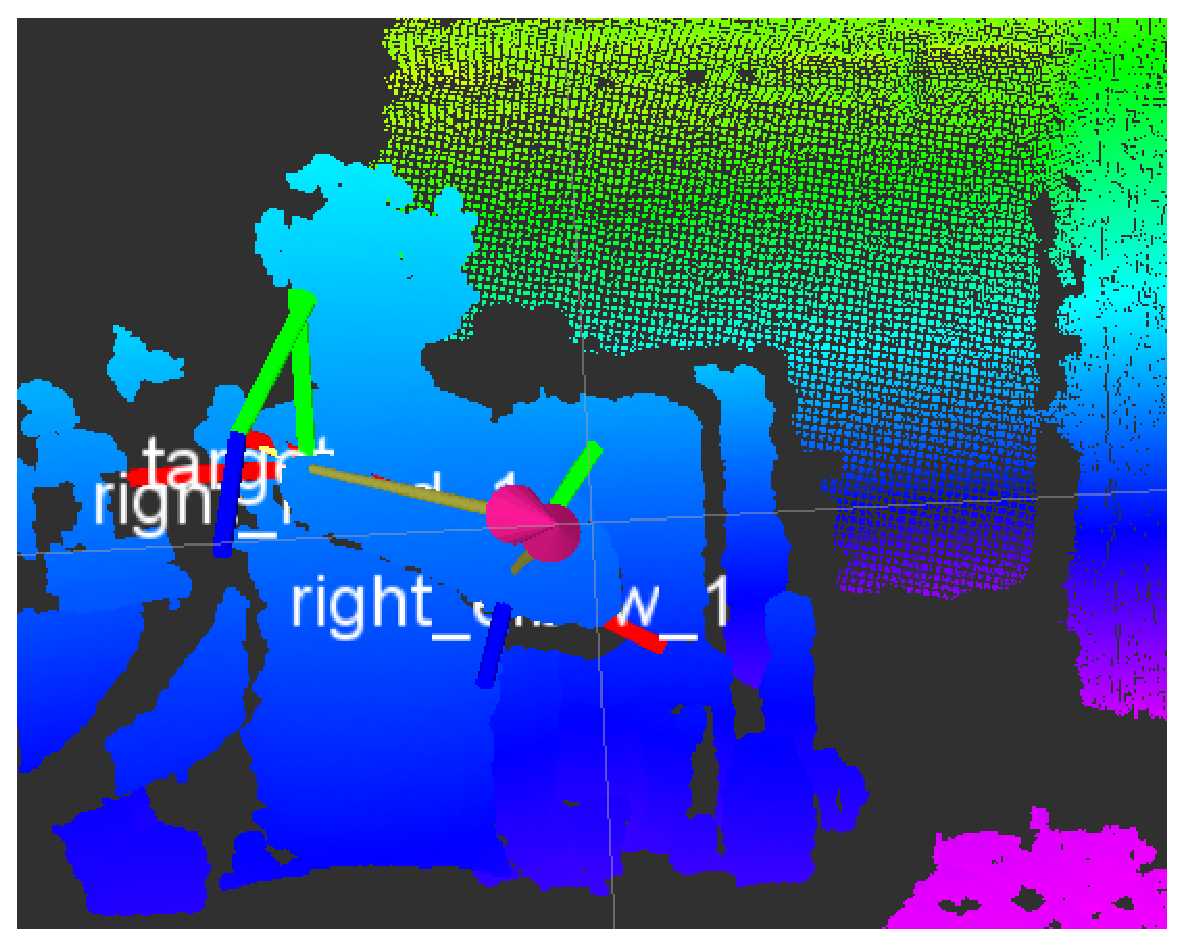
\includegraphics[width=0.48\textwidth]{figures/frames.eps}  
\caption{Display showing the center of the AoI (labelled "target") along with the detected hand and elbow centers.}
\label{fig:frames}
\end{wrapfigure}
\subsection{Segmentation} \label{sec:segmentation}
After identifying the AoI, Jarvis uses a set of heuristics to identify the target. Our application is geared towards soldering assistance, so the heuristic looks for a flat pcb board. It uses Random Sample Consensus (RANSAC) to fit a plane to the points in the AoI
\begin{equation} \label{eq:plane}
ax+by+cz+d=0 
\end{equation}
 and then filters out any point not on that plane. This procedure assumes that the target the largest plane in the small, floating AoI. While it puts restrictions on the target, it is able to adapt to boards of different sizes and shapes. This step can also be easily swapped out for a different heuristic-based segmentation depending on the application.  

\subsection{Grasp Generation}\label{sec:graspgen} 
Jarvis represents grasps as a coordinate frame with its origin at the target point and oriented so that its z axis points directly towards the gripper and the x axis is along the gripper's closing direction (figure \ref{fig:gripper}.) This representation assumes a simple pinch gripper, but could be used by more complicated grippers as well. 
\par Finding an appropriate grip requires finding both an orientation and a position. The planar shape of the target provides a useful constraint on the x axis of the grasp: the gripper will ideally close in a direction perpendicular to the plane. Thus the vector normal to the plane - $\hat{\textbf{n}}$ - found in \ref{sec:segmentation} defines the x axis of the grip.
\begin{equation}
\hat{\textbf{x}}_{\text{grasp}} = \hat{\textbf{n}}
\end{equation}
 Similarly, the human expectation that a handoff occurs on the opposite side of the target helps define the z axis. Jarvis uses the elbow-hand vector as the z axis of the grip so that the hand-off occurs with with robot arm as close to mirroring the human arm as possible. This orientation assumes that the grip will be roughly along the edge of the target that opposes the human's hand.
 \begin{equation}
\hat{\textbf{z}}_{\text{grasp}} = \hat{\textbf{v}}_{eh}
\end{equation}
The orientation's y component will point along the plane and can be found by taking the cross product of $\hat{\textbf{z}}$ and $\hat{\textbf{x}}$.
\begin{equation}
\hat{\textbf{y}}_{\text{grasp}} = \hat{\textbf{z}}_{\text{grasp}} \times \hat{\textbf{x}}_{\text{grasp}}
\end{equation}
\par To find a grip point that matches the orientation,  Jarvis first extends the elbow-hand vector by a constant that assures its end will reach beyond the edge of the target.
\begin{equation} \label{eq:vec_ext}
\textbf{v}_{eh}^* = 1.5 \textbf{v}_{eh}
\end{equation}
The point in the target cloud closest to the vector projected into the target plane (equation \ref{eq:plane}) is guaranteed to be an edge point of the target, if the target cloud has no extraneous points. 
\begin{equation} \label{eq:planar_proj}
\textbf{v}_{plane} = \textbf{v}_{eh}^* - 
				\left(\textbf{v}_{eh}^* \cdot \hat{\textbf{n}} \right) \hat{\textbf{n}}
\end{equation}

\begin{equation}
p_{\text{grasp}} = \operatorname*{arg\,min}_{p_i} \left(\,\norm{p_i - v_{eh}^*} | \,p_i \in \text{target cloud}\right)
\end{equation}
This search is performed by searching for the nearest neighbor to the extended elbow-hand vector in a k-d tree representation of the target cloud. 
\par The final grasp is defined by the coordinate frame $ \hat{\textbf{x}}_{\text{grasp}}, \hat{\textbf{y}}_{\text{grasp}}, \hat{\textbf{z}}_{\text{grasp}} $ and the point $p_{\text{grasp}}$.

\begin{wrapfigure}{r}{0.5\textwidth}
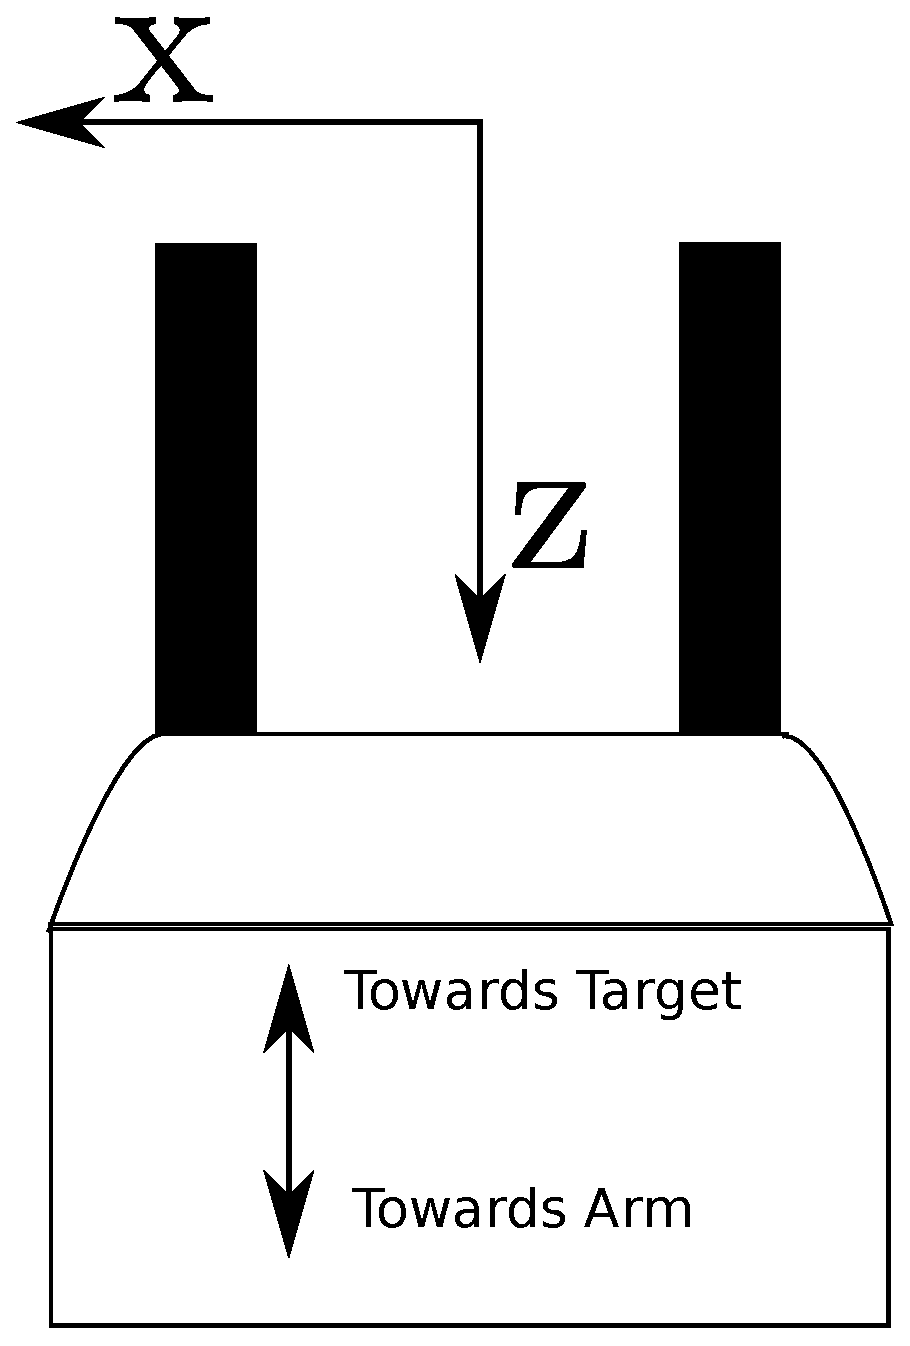
\includegraphics[width=0.48\textwidth]{figures/gripper_diagram.eps}  
\caption{Grip coordinate system}
\label{fig:gripper}
\end{wrapfigure}


\section{Discussion} \label{sec:discussion}
\par The collision avoidance algorithm does well when the skeleton tracker gives consistent output, but has a tendency to locate a 4cm forearm in the human's head when the skeleton tracker produces noisy data. These tracking problems can be avoided by standing an appropriate distance from the Kinect (~1-4m) and moving slowly. This suggests that future grip generators shouldn't rely on skeleton tracking data to ID human parts. One alternative method would be to use RGB data and OpenCV to either recognize hand colors %todo cite
or train a classifier to recognize the edges of the arm and hand and then project those pixels back onto their corresponding point cloud voxels in 3-space. Another alternative method is matching sets of segmented points to a preexisting model of an arm and hand.     

Approaches not used
\begin{itemize}
\item Creating a convex hull model for the object after planar segmentation
\item Implementing a kalman filter on the points in the object or
\item Running a filter on the plane coefficients
\end{itemize}

\par This method of grasp detection is slow for two major reasons: it performs 

\section{Bibliography}
\bibliographystyle{plain} 
\bibliography{bibliography}


\end{document}

